%==============================================================================
% Sjabloon poster bachproef
%==============================================================================
% Gebaseerd op document class `a0poster' door Gerlinde Kettl en Matthias Weiser
% Aangepast voor gebruik aan HOGENT door Jens Buysse en Bert Van Vreckem

\documentclass[a0,portrait]{hogent-poster}

% Info over de opleiding
\course{Bachelorproef}
\studyprogramme{toegepaste informatica}
\academicyear{2022-2023}
\institution{Hogeschool Gent, Valentin Vaerwyckweg 1, 9000 Gent}

% Info over de bachelorproef
\title{Optimalisatie van ERP (Enterprise resource planning) patchmanagement bij Managed Service Providers.}
\subtitle{Een diepgaande analyse van praktijken en efficiëntieverhogende maatregelen.}
\author{Gilles Detrooz}
\email{gilles.detrooz@student.hogent.be}
\supervisor{Marc Asselberg}
\cosupervisor{Kasper Heyndrickx (delaware)} 

% Indien ingevuld, wordt deze informatie toegevoegd aan het einde van de
% abstract. Zet in commentaar als je dit niet wilt.
\specialisation{Systeem- en Netwerkbeheer}
\keywords{operationele continuïteit, zorgvuldige planning, gefaseerde implementatie, fallbackstrategieën, systeemstoringen, communicatie, back-ups, veiligheid, stabiliteit}
\projectrepo{https://github.com/GillesDetr/latex-hogent-bachproef}

\begin{document}

\maketitle

\begin{abstract}
  Deze bachelorproef onderzoekt de optimalisatie van ERP (Enterprise Resource Planning) patchmanagement bij Managed Service Providers (MSP's). Het onderzoek is gericht op het identificeren en implementeren van efficiënte patchmanagementstrategieën om de downtime te minimaliseren en de beveiliging te maximaliseren. Door middel van literatuurstudie, casestudies en interviews met experts worden de huidige praktijken geanalyseerd en geavanceerde tools zoals Avantra geëvalueerd. De resultaten tonen aan dat geautomatiseerde patchingtools significant bijdragen aan de efficiëntie en veiligheid van ERP-systemen. De aanbevelingen omvatten de implementatie van geavanceerde tools, duidelijke communicatiestrategieën en continue training voor IT-professionals.
\end{abstract}

\begin{multicols}{2} % This is how many columns your poster will be broken into, a portrait poster is generally split into 2 columns

\section{Introductie}
ERP-systemen vormen de ruggengraat van de IT-infrastructuur in veel grote en middelgrote bedrijven. Ze zijn essentieel voor het stroomlijnen van bedrijfsprocessen en het verbeteren van operationele efficiëntie. Echter, deze systemen zijn complex en vereisen regelmatig onderhoud, waaronder patchmanagement, om beveiligingsrisico's te minimaliseren en de prestaties te optimaliseren. Managed Service Providers (MSP's) spelen een cruciale rol in het beheer van deze systemen voor hun klanten. Dit onderzoek richt zich op het optimaliseren van patchmanagementpraktijken binnen MSP's die SAP ERP-systemen beheren. De focus ligt op het analyseren van de huidige praktijken, het identificeren van inefficiënties en het voorstellen van verbeteringen door middel van geavanceerde tools en technieken.

\section{Methodologie}
De onderzoeksmethode voor deze bachelorproef bestaat uit vijf fasen. In Fase 1 wordt een uitgebreide literatuurstudie uitgevoerd om inzicht te krijgen in de huidige staat van ERP-patchmanagement bij managed service providers. Hierbij worden academische publicaties en vakliteratuur geanalyseerd om bestaande procedures en uitdagingen te identificeren. Fase 2 richt zich op een specifieke casestudy bij een managed service provider, waarbij 
het patchmanagementproces gedetailleerd in kaart wordt gebracht met behulp van een BPMN-schema. Deze fase duurt vier weken. In Fase 3 worden interviews gehouden met ERP-experts om een dieper inzicht te krijgen in de tactieken en mogelijke verbeteringen van het patchmanagementproces. Deze fase neemt drie weken in beslag. Fase 4 analyseert beschikbare tools en praktijken voor ERP-patchmanagement, met een focus op hoe deze het proces kunnen verbeteren. Deze fase 
duurt ook drie weken. Tot slot worden in Fase 5 de resultaten van de literatuurstudie, casestudy en interviews samengebracht. Conclusies worden getrokken en specifieke adviezen geformuleerd om de effectiviteit van ERP-patchmanagement in organisaties te verbeteren. Deze fase duurt twee weken.


\section{Case study}
Een case study werd uitgevoerd bij een MSP die SAP ERP-systemen beheert voor klanten in verschillende sectoren. Het doel van de case study was om inzicht te krijgen in de huidige patchmanagementpraktijken en kijken waar men nog met uitdagingen zit en waar er tijd kan worden bespaard. Uit dit proces werd een BMPN-schema gemaakt om de huidige situatie in kaart te brengen. Door dit schema krijgen we een globaal beeld en kan er gekeken worden waar er nog verbeteringen mogelijk zijn.
  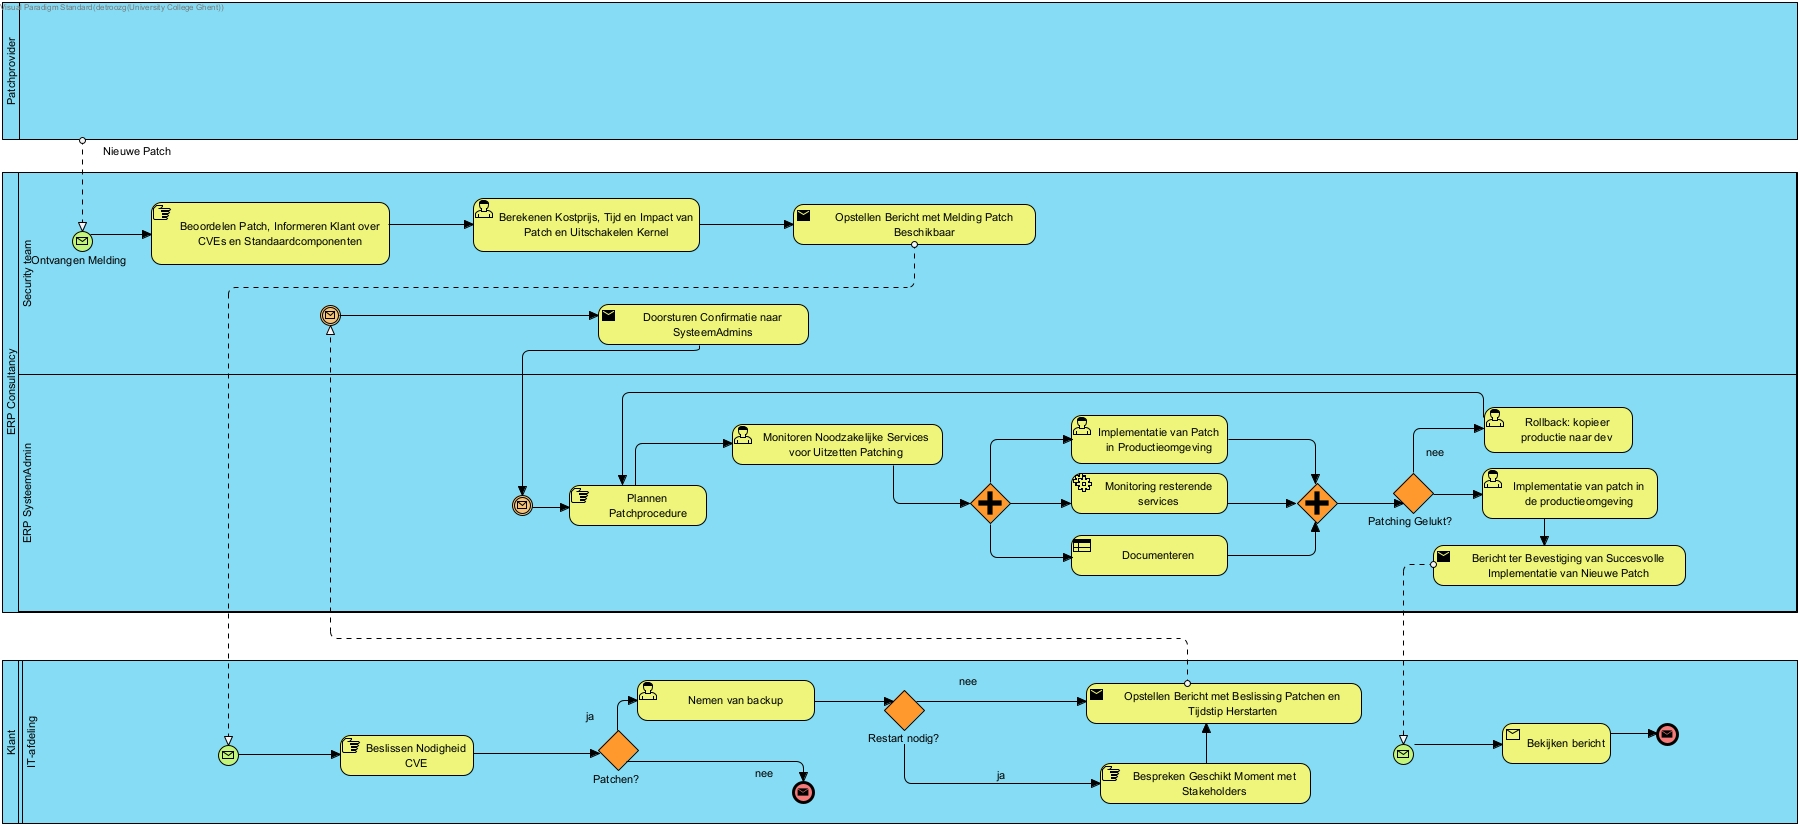
\includegraphics[width=1.0\linewidth]{huidigesituatie.jpg}
  \captionof{figure}{Huidige situatie van kernel-patchmanagement bij de MSP.}
\end{center}

\section{Conclusies}
Een case study bij een managed service provider toonde aan dat het ERP patchproces aanzienlijk verbeterd kan worden door automatisering. Tools zoals Avantra kunnen kernel patching efficiënt uitvoeren, wat aanzienlijke tijdsbesparing oplevert voor bedrijven die veel systemen beheren. Echter, de implementatie van dergelijke tools kost tijd en is niet gratis. Het onderzoek benadrukt het belang van goede communicatie en geautomatiseerde tools voor effectieve patching. Cloudgebaseerde ERP-systemen bieden voordelen zoals schaalbaarheid en kosteneffectiviteit. De toekomst van patchmanagement ziet er veelbelovend uit met de opkomst van AI en machine learning, hoewel implementatie en ethische overwegingen aandacht vereisen. Best practices zoals systematisch patchbeheer en voorafgaande tests zijn essentieel voor succes.

\section{Toekomstig onderzoek}
Er moet verder onderzocht worden hoe AI geïntegreerd kan worden in dit proces om de communicatie te verbeteren en de downtime te minimaliseren. Dit kan bijvoorbeeld door de agenda's van de betrokken partijen te synchroniseren en automatisch updates te plannen op momenten dat de impact minimaal is. Daarnaast is het belangrijk om de ethische aspecten van AI in patchmanagement te onderzoeken, zoals privacy en veiligheid. Verder onderzoek kan zich richten op de implementatie van geavanceerde tools zoals Avantra en de impact ervan op de efficiëntie en veiligheid van ERP-systemen.


\end{multicols}
\end{document}